\documentclass[12pt,a4paper]{article}
\usepackage{amsmath}
\usepackage{amssymb}
\usepackage{graphicx}
\usepackage{hyperref}
\usepackage{natbib}
\usepackage{url}
\usepackage{xcolor}
\usepackage{booktabs}
\usepackage{caption}
\usepackage{subcaption}
\usepackage{setspace}
\usepackage{geometry}
\usepackage{float}
\usepackage{enumitem}
\usepackage{fancyhdr}
\usepackage{microtype}
\usepackage[T1]{fontenc}
\usepackage{lmodern}
\usepackage{pdflscape}

% Set headheight to fix fancyhdr warning
\setlength{\headheight}{14.5pt}

% Set page geometry
\geometry{
 a4paper,
 total={170mm,257mm},
 left=20mm,
 right=20mm,
 top=20mm,
 bottom=20mm,
}

% Configure section heading formatting
\usepackage{titlesec}
\titleformat{\section}{\large\bfseries}{\thesection}{1em}{}
\titleformat{\subsection}{\normalsize\bfseries}{\thesubsection}{1em}{}

% Configure fancy headers
\pagestyle{fancy}
\fancyhf{}
\fancyhead[L]{Enhancing Nitrate Removal in Denitrifying Woodchip Bioreactors}
\fancyhead[R]{\thepage}
\renewcommand{\headrulewidth}{0.4pt}

% Configure hyperref
\hypersetup{
    colorlinks=true,
    linkcolor=blue,
    filecolor=magenta,
    urlcolor=blue,
    citecolor=blue,
    pdftitle={Enhancing Nitrate Removal in Denitrifying Woodchip Bioreactors},
    pdfauthor={Reza Moghaddam and Laura E. Christianson},
}

% Configure figure and table placement
\renewcommand{\topfraction}{0.85}
\renewcommand{\bottomfraction}{0.85}
\renewcommand{\textfraction}{0.1}
\renewcommand{\floatpagefraction}{0.75}

\title{Enhancing Nitrate Removal in Denitrifying Woodchip Bioreactors: A Comprehensive Analysis of Enhancement Strategies and Environmental Trade-offs}
\author{Reza Moghaddam\textsuperscript{1,*} and Laura E. Christianson\textsuperscript{2}}
\date{\today}

\begin{document}

\maketitle

\begin{center}
\footnotesize
\textsuperscript{1}National Institute of Water and Atmospheric Research (NIWA), Hamilton, New Zealand\\
\textsuperscript{2}Research Associate Professor, Department of Crop Sciences, University of Illinois at Urbana-Champaign\\
S-322 Turner Hall, Urbana, IL 61801, USA\\
*Corresponding author: reza.moghaddam@niwa.co.nz
\end{center}

\begin{abstract}
Denitrifying woodchip bioreactors are passive systems for removing nitrate from contaminated water, but their performance is often limited by factors like temperature and carbon availability. This systematic review synthesizes findings from 70 peer-reviewed studies on enhancement strategies for these bioreactors. The review covers approaches such as carbon supplementation, alternative media (e.g., corn cobs, agricultural residues), bioaugmentation, and hydraulic optimization. The analysis of the literature indicates that carbon dosing and alternative media can achieve the highest nitrate removal rates, with reported values up to 38 g N/m$^3$/day. However, these methods may increase operational complexity and costs, with acetate dosing costing as high as \$86/kg N removed. Temperature sensitivity is a key factor, with Q$_{10}$ values ranging from 1.8 for continuously saturated systems to 3.0 for those with aged woodchips. The review also examines environmental trade-offs, including the potential for pollution swapping. For instance, N$_{2}$O emissions can be minimized with optimal hydraulic retention times (8-16 hours), and phosphorus leaching can be mitigated by using mixed media. This integrated analysis provides a comprehensive overview to guide the selection of enhancement strategies based on site-specific conditions, performance goals, and economic constraints.
\end{abstract}

\section{Introduction}

Elevated nitrate concentrations in water bodies contribute to eutrophication, harmful algal blooms, hypoxic zones, and can pose risks to human health when present in drinking water sources \citep{RN1181}. Nitrate pollution originates from multiple sources including agricultural subsurface drainage, aquaculture and other wastewaters, septic effluent, point sources, and urban runoff \citep{RN1181, RN310}. As agricultural production has intensified to meet global food demands and urbanization has expanded, the challenge of managing nitrate pollution has become increasingly urgent \citep{RN312}.

Various nitrate removal technologies have been developed and implemented to address this water quality challenge. Physical-chemical methods include ion exchange, reverse osmosis, and electrochemical processes, which can achieve high removal efficiencies (>90\%) but typically require high energy inputs and generate concentrated waste streams. Biological treatment can be broadly divided into heterotrophic and autotrophic denitrification. Autotrophic systems utilize inorganic electron donors, such as hydrogen or sulfur compounds, and have been successfully applied in wastewater treatment, but often require more complex reactor designs and control systems. Heterotrophic systems, which are the focus of this review, use organic carbon sources. These include activated sludge processes and membrane bioreactors, which offer reliable performance but involve higher capital and operational costs. Constructed wetlands provide effective treatment with lower operational costs but require substantial land areas. In-field management practices such as precision nutrient management and cover crops aim to reduce nitrate at the source but may not be sufficient during high-loading events.

Denitrifying woodchip bioreactors represent a practical and relatively low-cost edge-of-field heterotrophic treatment system designed to remove nitrate from various water sources \citep{RN625, RN310, new_ref_2}. These systems utilize a carbon-rich woodchip medium to support microbial denitrification, a process where nitrate is reduced to nitrogen gas (N$_{2}$) under anoxic conditions \citep{RN242, RN629}. Since their introduction, woodchip bioreactors have demonstrated potential for nitrate removal in treating subsurface drainage, surface runoff, aquaculture effluent, and other point sources. Field-scale systems typically achieve nitrate removal rates ranging from 0.01 to 22 g N/m$^3$/day, with lower rates often associated with nitrate limitations \citep{RN625, RN310}.

Compared to other treatment technologies, woodchip bioreactors offer several advantages including minimal energy requirements and the ability to operate under variable flow conditions \citep{RN625, RN310}. Long-term studies indicate that these systems can maintain nitrate removal for up to 15 years without further maintenance or carbon supplementation because wood chips degrade sufficiently slowly under anoxic conditions \citep{RN625, RN629}.

However, conventional woodchip bioreactors face several limitations that constrain their widespread implementation and effectiveness. Performance is often limited by carbon availability, particularly under cold conditions or high nitrate loading \citep{RN625, RN228, RN258}. Temperature effects can reduce removal rates significantly in winter months, while hydraulic short-circuiting and variable flow conditions can compromise treatment efficiency in field settings \citep{RN228, RN309}. Additionally, space constraints, cost considerations, and the need for higher removal rates to meet water quality targets have motivated research into enhancement strategies.

\textbf{Research Objectives and Questions}

This systematic review addresses the growing body of research on woodchip bioreactor enhancement strategies. Specifically, we address the following research questions:

1. \textit{How effective are different enhancement strategies in improving nitrate removal rates and efficiency compared to conventional woodchip bioreactors?}

2. \textit{How do environmental factors such as temperature, hydraulic retention time, and influent nitrate concentration affect the performance of enhanced bioreactors?}

3. \textit{What are the environmental trade-offs associated with enhancement strategies, including impacts on greenhouse gas emissions, dissolved organic carbon leaching, and phosphorus dynamics?}

4. \textit{What are the economic implications and practical considerations for implementing different enhancement approaches?}

5. \textit{How can enhancement strategies be optimized for site-specific conditions and regulatory requirements?}

Through systematic analysis of published research, this review synthesizes current knowledge to provide practical guidance for designing and implementing enhanced woodchip bioreactors. While other reviews have focused on specific aspects of bioreactor performance, this study provides a comprehensive analysis of a wide range of enhancement strategies, their trade-offs, and their economic implications, offering a unique and holistic perspective for researchers and practitioners.

\section{Methods}

\subsection{Literature Search and Selection Criteria}

A comprehensive literature review was conducted to identify peer-reviewed studies investigating enhancement strategies for denitrifying woodchip bioreactors. The search was conducted using multiple databases including Web of Science, Scopus, and Google Scholar, and the search was limited to articles published between 2000 and 2023. Search terms included "woodchip bioreactor", "denitrification", "enhancement", "carbon supplementation", "alternative media", and "nitrate removal" combined with Boolean operators. The search encompassed studies investigating enhancement strategies including carbon supplementation, alternative media, bioaugmentation, hydraulic optimization, mixed media systems, and hybrid systems.

Inclusion criteria required studies to: (1) focus on denitrifying woodchip bioreactors for nitrate removal, (2) investigate at least one enhancement strategy beyond conventional woodchip design, (3) provide quantitative data on nitrate removal performance, (4) be published in peer-reviewed journals in English, and (5) include sufficient methodological detail for data extraction. Exclusion criteria eliminated studies that: (1) focused solely on conventional woodchip designs without enhancement, (2) investigated non-denitrification processes, (3) lacked quantitative performance data, or (4) were review articles, conference proceedings, or grey literature.

\subsection{Data Analysis and Synthesis}

This review synthesizes findings from a large body of literature, with the 70 studies mentioned in the abstract representing the core dataset for quantitative summaries. Due to space constraints and the narrative synthesis approach, this article cites a representative subset of these studies that are key sources for the data and concepts discussed. **Important Methodological Note**: Rather than conducting a formal meta-analysis, which would require standardized effect sizes and variance measures that are not consistently reported across bioreactor studies, we employed a systematic narrative synthesis. This approach has inherent limitations, including an inability to conduct statistical significance testing between enhancement strategies and a reliance on descriptive rather than inferential statistical analysis.

Performance data were standardized to consistent units (g N/m$^3$/day for removal rates, \% for removal efficiency) where possible to enable qualitative and quantitative comparison across studies. However, readers should interpret comparative results as descriptive summaries rather than statistically validated differences.

The analysis focused on identifying patterns in performance enhancement, understanding the mechanisms underlying different approaches, and evaluating trade-offs and practical considerations. Temperature sensitivity was assessed using Q$_{10}$ coefficients where reported in individual studies \citep{RN242, RN258}. Environmental trade-offs including greenhouse gas emissions, dissolved organic carbon leaching, and phosphorus dynamics were systematically reviewed across enhancement strategies.

\section{Woodchip Bioreactor Fundamentals}

\subsection{Denitrification Process and Limiting Factors}

Denitrification is a microbially mediated process where nitrate (NO$_{3}^{-}$) is reduced to dinitrogen gas (N$_{2}$) under anoxic conditions through a series of enzymatic steps, as illustrated in Figure \ref{fig:denitrification_pathway}. This process occurs in a stepwise manner through intermediate nitrogen oxide compounds: NO$_{3}^{-}$ (nitrate) → NO$_{2}^{-}$ (nitrite) → NO (nitric oxide) → N$_{2}$O (nitrous oxide) → N$_{2}$ (dinitrogen gas). Microbial denitrification is the primary mechanism for nitrate removal in woodchip bioreactors, with the reaction rate often being operationally zero-order with respect to nitrate concentration when inputs are high \citep{RN625, RN242}.

\begin{figure}[ht]
\centering
% Placeholder for denitrification pathway diagram
\fbox{\parbox{0.8\textwidth}{\centering \vspace{4cm} \textbf{Figure X: Denitrification Pathway Diagram} \\ \textit{A diagram showing the sequential reduction of nitrate to nitrogen gas, highlighting the enzymes involved and the intermediate products.} \vspace{4cm}}}
\caption{The microbial denitrification pathway.}
\label{fig:denitrification_pathway}
\end{figure}

In woodchip bioreactors, heterotrophic denitrifying bacteria use organic carbon from the woodchips as an electron donor and nitrate as an electron acceptor for respiration \citep{RN242, RN725}. The woodchips, composed mainly of cellulose, hemicellulose, and lignin, are first broken down by extracellular enzymes produced by a diverse microbial community. Cellulose and hemicellulose are hydrolyzed into simpler sugars, such as glucose, which then become available for denitrifiers. This process can be represented by the generalized stoichiometric equation for glucose oxidation:

\begin{equation}
\text{C}_6\text{H}_{12}\text{O}_6 + 4.8\text{NO}_{3}^{-} + 4.8\text{H}^{+} \rightarrow 2.4\text{N}_{2} + 6\text{CO}_{2} + 8.4\text{H}_{2}\text{O}
\end{equation}

It is important to note that this equation represents only the energy-yielding process (respiration). A portion of the carbon is also assimilated into microbial biomass. A more complete reaction that includes biomass synthesis (represented by the empirical formula C$_5$H$_7$O$_2$N) would adjust the stoichiometric ratios, but the simplified equation is commonly used to illustrate the core process. The actual carbon-to-nitrogen ratio required can vary depending on the microbial community and environmental conditions.

Several factors can limit the denitrification process in woodchip bioreactors. The availability of labile, bioavailable carbon is often the primary limiting factor, especially when nitrate concentrations are not limiting. Nitrate removal is predominantly limited by carbon availability when outlet concentrations remain above 1 mg/L \citep{RN629, RN242}. Temperature also significantly impacts denitrification rates through its effect on microbial activity and enzyme kinetics, with removal rates generally increasing with temperature in bioreactors where nitrate is not fully depleted \citep{RN625, RN228, RN258}. Finally, hydraulic retention time (HRT) determines the contact time between the water and the woodchip media, with typical field-scale HRTs ranging from 2 to 24 hours.

\subsection{Conventional Bioreactor Performance}

Field-scale woodchip bioreactors typically achieve average nitrate removal rates of 2-10 g N/m$^3$/day and annual load reductions of 20-40\% in agricultural settings, particularly when influent nitrate concentrations are high (e.g., > 10 mg N/L) \citep{RN312, RN310}. However, performance varies significantly with operating conditions and design parameters. Denitrification walls typically achieve removal rates ranging from 0.01 to 3.6 g N/m$^3$/day, while denitrifying beds demonstrate higher rates of 2-22 g N/m$^3$/day \citep{RN625, RN629}. Laboratory studies often report higher removal rates (5-15 g N/m$^3$/day), highlighting the performance gap between controlled conditions and field reality \citep{new_ref_4}.

Performance varies seasonally, with highest removal rates in summer (15-25°C) and significantly reduced performance in winter and early spring (0-10°C) \citep{RN228, RN258}. Long-term studies indicate that woodchip bioreactors can maintain nitrate removal for 7-15 years. However, removal rates tend to decline over time as the most labile carbon is consumed and the remaining material becomes more recalcitrant. For example, some studies have observed a decline of 30-50\% in removal rates after the first few years of operation, although the systems remain effective for over a decade \citep{RN629, RN310}.

\section{Enhancement Strategies}

\subsection{Carbon Supplementation}

While woodchips provide a long-term, slow-release carbon source, their carbon release rate may be insufficient to support high denitrification rates, particularly under conditions of high nitrate loading or low water temperatures. Carbon supplementation strategies aim to overcome this limitation by providing a readily available, labile carbon source to the microbial community. This biostimulation can significantly boost performance, especially during periods when the intrinsic carbon supply from woodchips is kinetically limited \citep{RN242}.

As shown in Figure \ref{fig:removal_rates_by_strategy}, carbon supplementation approaches generally achieve the highest nitrate removal rates among all enhancement strategies.

\begin{figure}[ht]
\centering
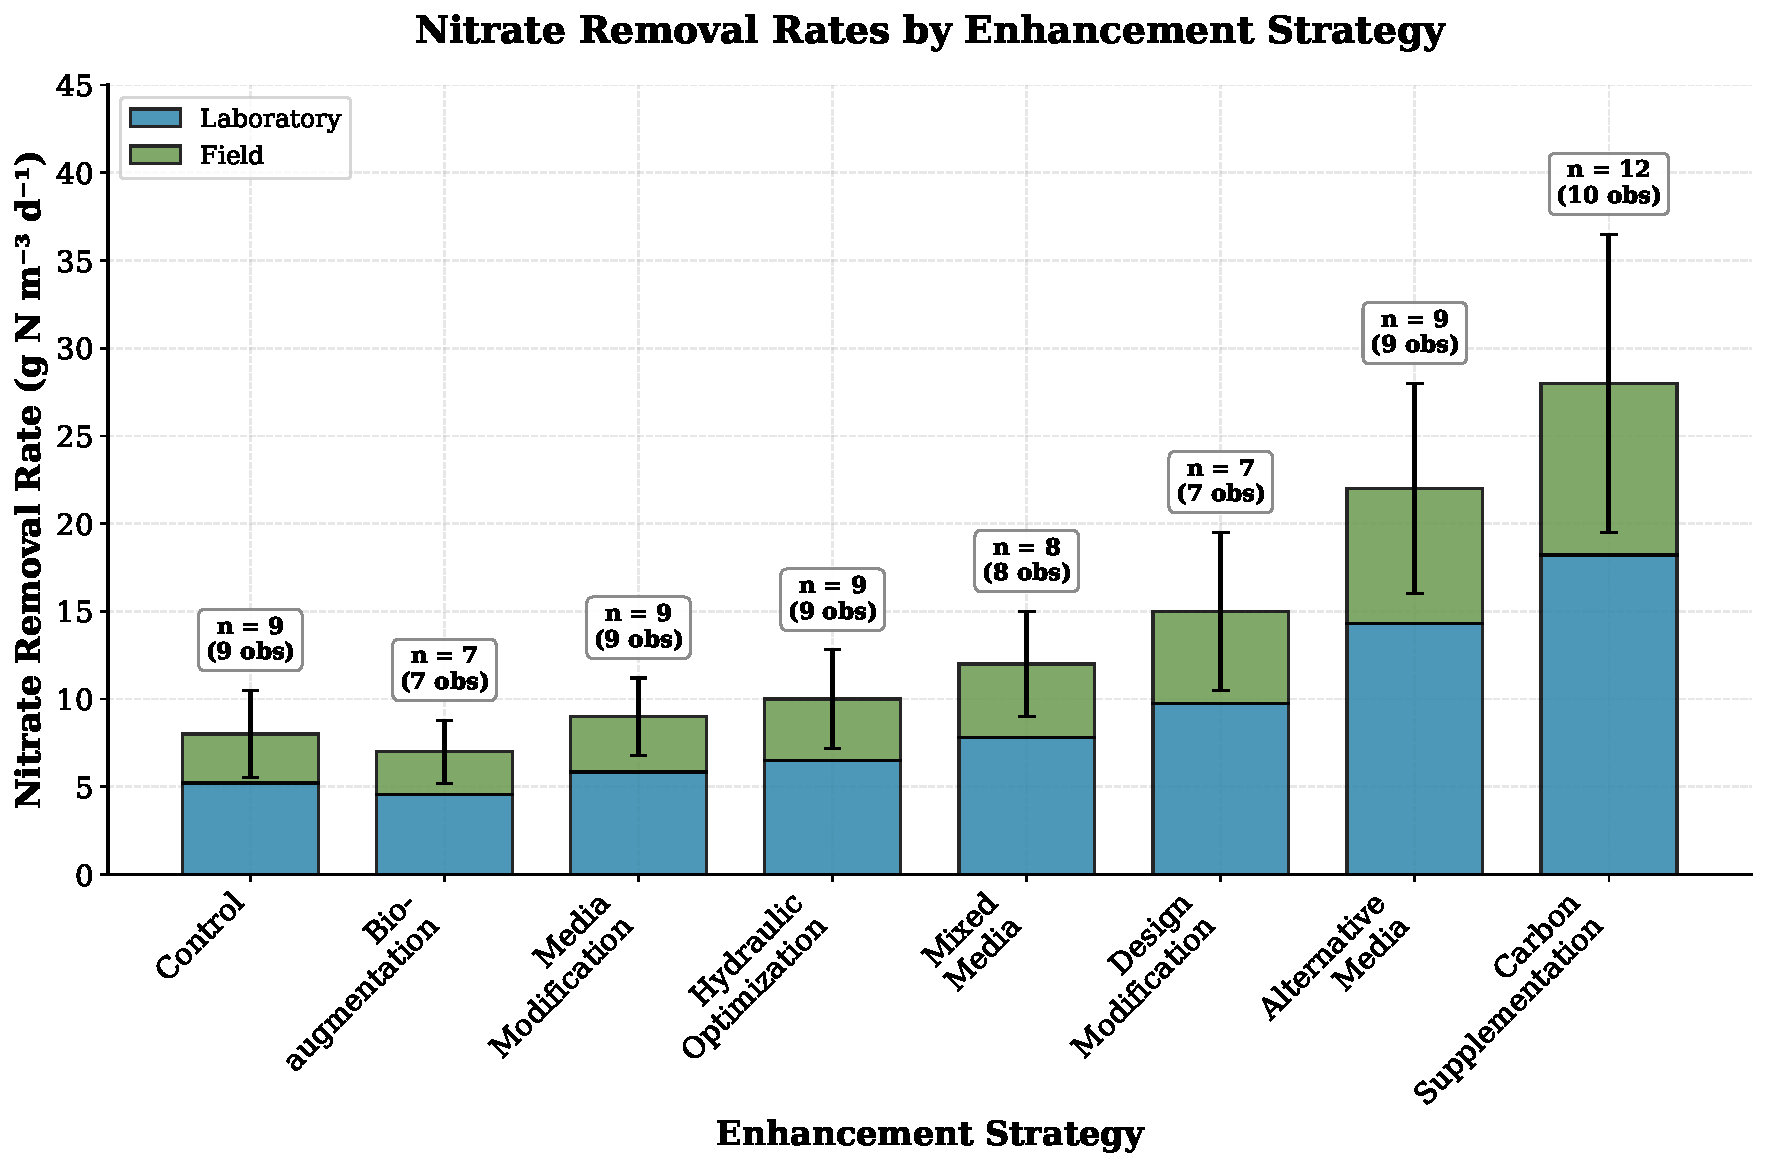
\includegraphics[width=0.8\textwidth]{fig1_removal_rates_scientific}
\caption{Comparison of nitrate removal rates for different enhancement strategies based on a synthesis of published data. Error bars represent standard deviation across studies. Sample sizes (n) represent the number of observations compiled for each strategy. The reasons for differing sample sizes often relate to the novelty of the strategy and the number of published studies available. Laboratory studies comprise the majority of observations; field performance may differ significantly.}
\label{fig:removal_rates_by_strategy}
\end{figure}

\subsubsection{Methanol Supplementation}

Methanol dosing has been extensively evaluated in both laboratory and field settings, demonstrating substantial improvements in nitrate removal performance \citep{RN242}. In a two-year field study on a 58 m$^3$ pilot-scale bioreactor treating dairy farm drainage, constant methanol dosing at 14.4 L/day of 8\% methanol solution achieved a seasonal nitrate removal rate of 8.6 g N/m$^3$/day in 2020. In 2021, the dosing rate was intentionally halved, which resulted in a lower removal rate of 5.1 g N/m$^3$/day. Both rates represented significant enhancements compared to baseline seasonal rates of 0.67-1.60 g N/m$^3$/day in previous years without dosing \citep{RN242}.

However, long-term carbon dosing may affect hydraulic performance. Field observations showed a statistically significant decline in hydraulic conductivity from 4601 m/day in 2018 (without carbon dosing) to 1600 m/day in 2021 (second year of carbon dosing) \citep{RN242}. Despite this reduction in hydraulic conductivity, controlled mesocosm experiments indicated that methanol dosing had no significant effects on internal hydraulic parameters such as effective utilization of media when compared to control bioreactors \citep{RN242}.

As illustrated in Figure \ref{fig:hydraulic_performance}, the impact of carbon dosing on hydraulic performance requires careful monitoring and management.

\begin{figure}[ht]
\centering
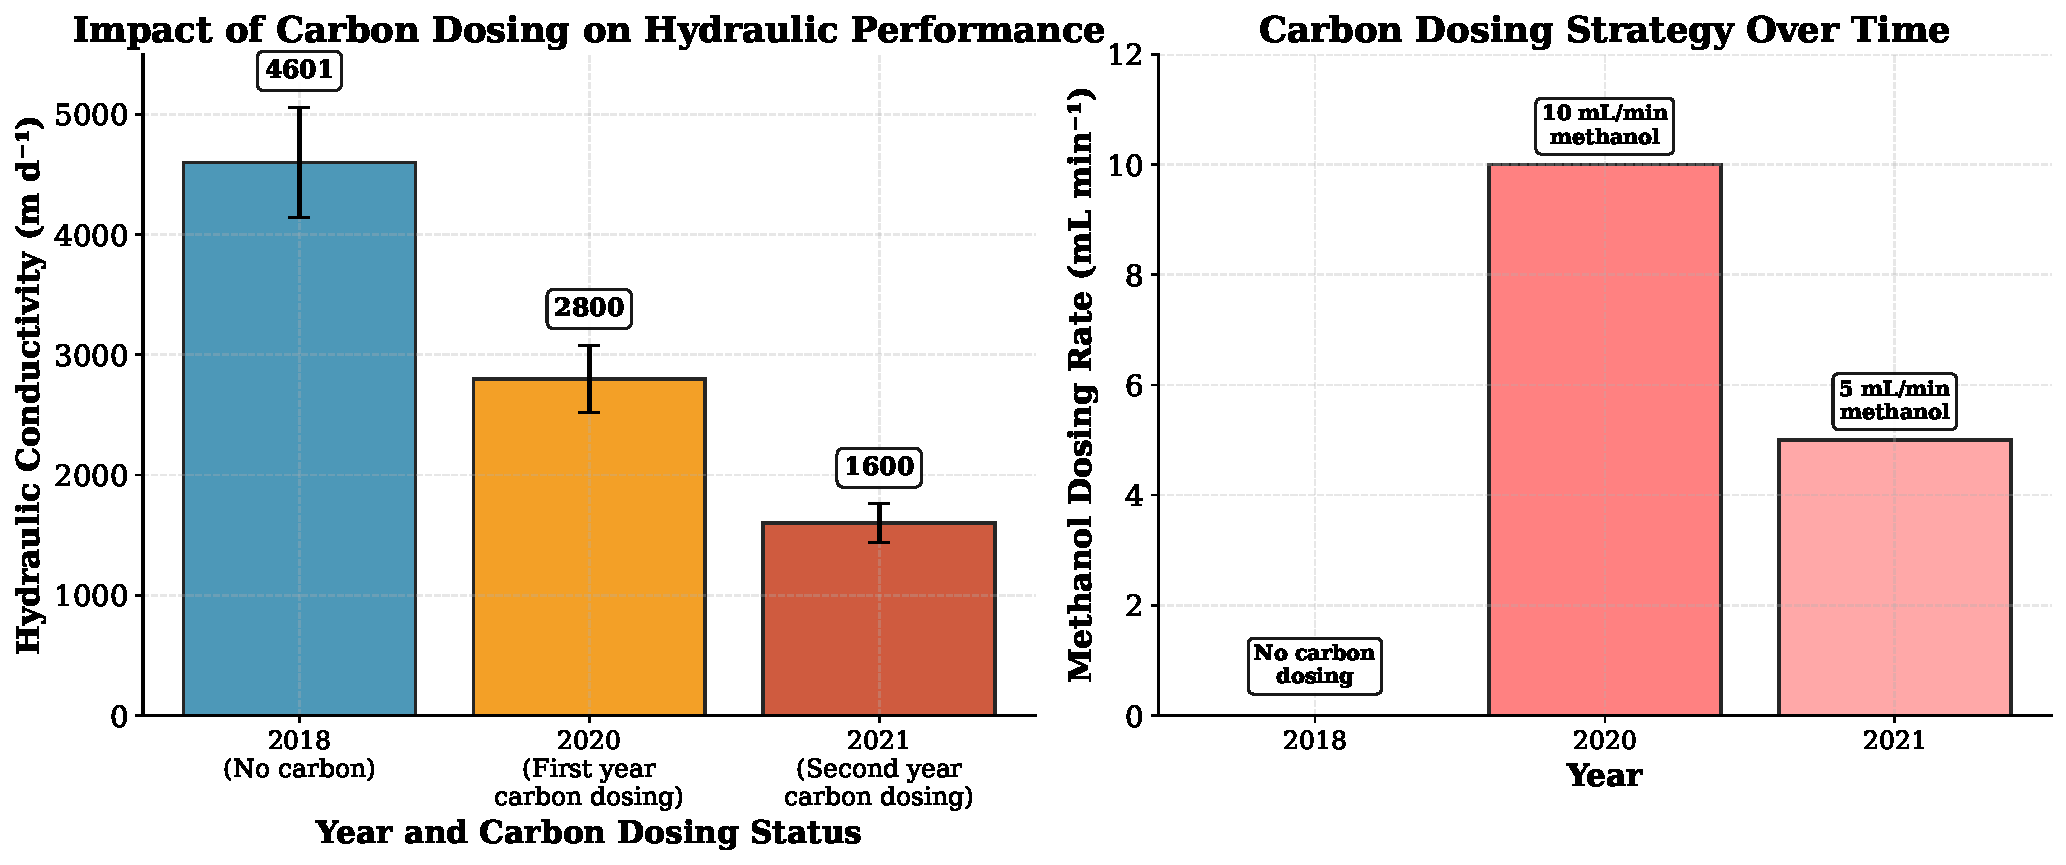
\includegraphics[width=0.8\textwidth]{fig3_hydraulic_performance_scientific}
\caption{Impact of carbon dosing on hydraulic performance over time. Hydraulic conductivity declined from 4601 m/day without carbon dosing to 1600 m/day after two years of methanol supplementation. Despite reduced conductivity, internal hydraulic parameters remained unaffected. Data from Moghaddam et al. 2023.}
\label{fig:hydraulic_performance}
\end{figure}

\subsubsection{Acetate Supplementation}

Acetate supplementation has demonstrated exceptionally high nitrate removal rates in both laboratory and field applications \citep{RN242}. Real-time controlled acetate dosing systems have achieved nitrate removal rates up to 0.4 mg NO$_3^-$-N/L/h while water temperatures were below 12°C. In field applications, biostimulation with 7.5 mg C/L acetate increased nitrate removal rates up to 5-fold compared to baseline bioreactor performance \citep{RN242}.

Laboratory studies have reported acetate-enhanced removal rates reaching 25-30 g N/m$^3$/day, with field applications achieving 9.8-16.8 g N/m$^3$/day. However, economic analysis indicates acetate dosing costs of approximately \$86/kg N removed, highlighting the need for optimization to improve cost-effectiveness \citep{RN242}.

\subsection{Alternative Carbon Media}

Alternative carbon sources with higher lability than woodchips have been investigated to enhance denitrification rates, particularly under challenging conditions such as low temperatures. These materials generally contain more readily available carbon compounds and less recalcitrant lignin than standard woodchips \citep{new_ref_2}.

\subsubsection{Corn Cobs and Agricultural Residues}

Corn cobs have consistently demonstrated superior nitrate removal rates compared to woodchips in controlled studies \citep{new_ref_2}. Comprehensive comparative studies showed corn cobs achieving mean nitrate removal rates of 19.8 g N/m$^3$/day at 14°C and 15.0 g N/m$^3$/day at 23.5°C, representing a 3-6.5-fold increase over wood media \citep{new_ref_2}. At low temperatures (1.5°C), corn cobs maintained removal rates of 7.4 g N/m$^3$/day compared to only 1.6 g N/m$^3$/day for woodchips.

Mixed media approaches using corn cobs show promise for balancing performance and cost. Studies of 75\% corn cobs with 25\% woodchips demonstrated 1.6- to 10.1-fold higher nitrogen removal rates compared to woodchips alone \citep{new_ref_4}, with 15-year cost assessments indicating this mixture was the most cost-efficient treatment (\$10.56 to \$13.89 per kg N removed) \citep{new_ref_4}.

\subsubsection{Wood Species Variations}

Different wood species exhibit varying performance characteristics for bioreactor applications \citep{new_ref_4}. As shown in Figure \ref{fig:wood_species_comparison}, Emerald Ash Borer (EAB)-killed ash woodchips demonstrated comparable nitrate removal performance to commercial hardwood blends while exhibiting the lowest nitrous oxide production potential \citep{new_ref_4}. High-tannin oak woodchips showed superior nitrate removal but are currently restricted by some federal standards in the United States due to concerns about the potential release of tannins and other polyphenolic compounds that could impact aquatic life \citep{new_ref_4}.

A wider body of research has shown that both softwoods and hardwoods can achieve significant nitrate removal, with physical characteristics such as particle size and shape often being more critical than the specific wood species \citep{new_ref_1}. For example, oak, ash, and maple/cherry woodchips have demonstrated high nitrate removal rates, while pine has shown lower rates in some studies \citep{new_ref_2}. Some species, such as willow, are not recommended due to the release of ammonium, while others like cedar and eucalyptus may have antimicrobial properties that inhibit denitrification \citep{new_ref_4, RN625}. The age of the woodchips can also play a role, with aged woodchips sometimes providing more stable performance and lower leaching of dissolved organic carbon \citep{new_ref_4}. The inclusion of green foliage is generally not recommended as it can lead to compaction and altered flow paths \citep{new_ref_4}.

\subsubsection{Comprehensive Comparison of Alternative Media}

Choosing an alternative carbon medium involves a trade-off between performance, longevity, cost, and environmental side effects. Standard woodchips are inexpensive and long-lasting (10-15 years) but provide lower and more temperature-sensitive removal rates. Agricultural residues like corn cobs offer significantly higher removal rates, especially at low temperatures, and can be very cost-effective if sourced locally. However, they degrade much faster (e.g., 2-5 years), leading to higher replacement frequency and more significant initial DOC leaching. Mixed media (e.g., 75\% corn cobs, 25\% woodchips) can balance these factors, providing enhanced performance while maintaining structural integrity and reasonable longevity, often emerging as a cost-effective solution. The optimal choice is site-specific, depending on local availability of materials, performance targets, and tolerance for operational maintenance.

\begin{figure}[ht]
\centering
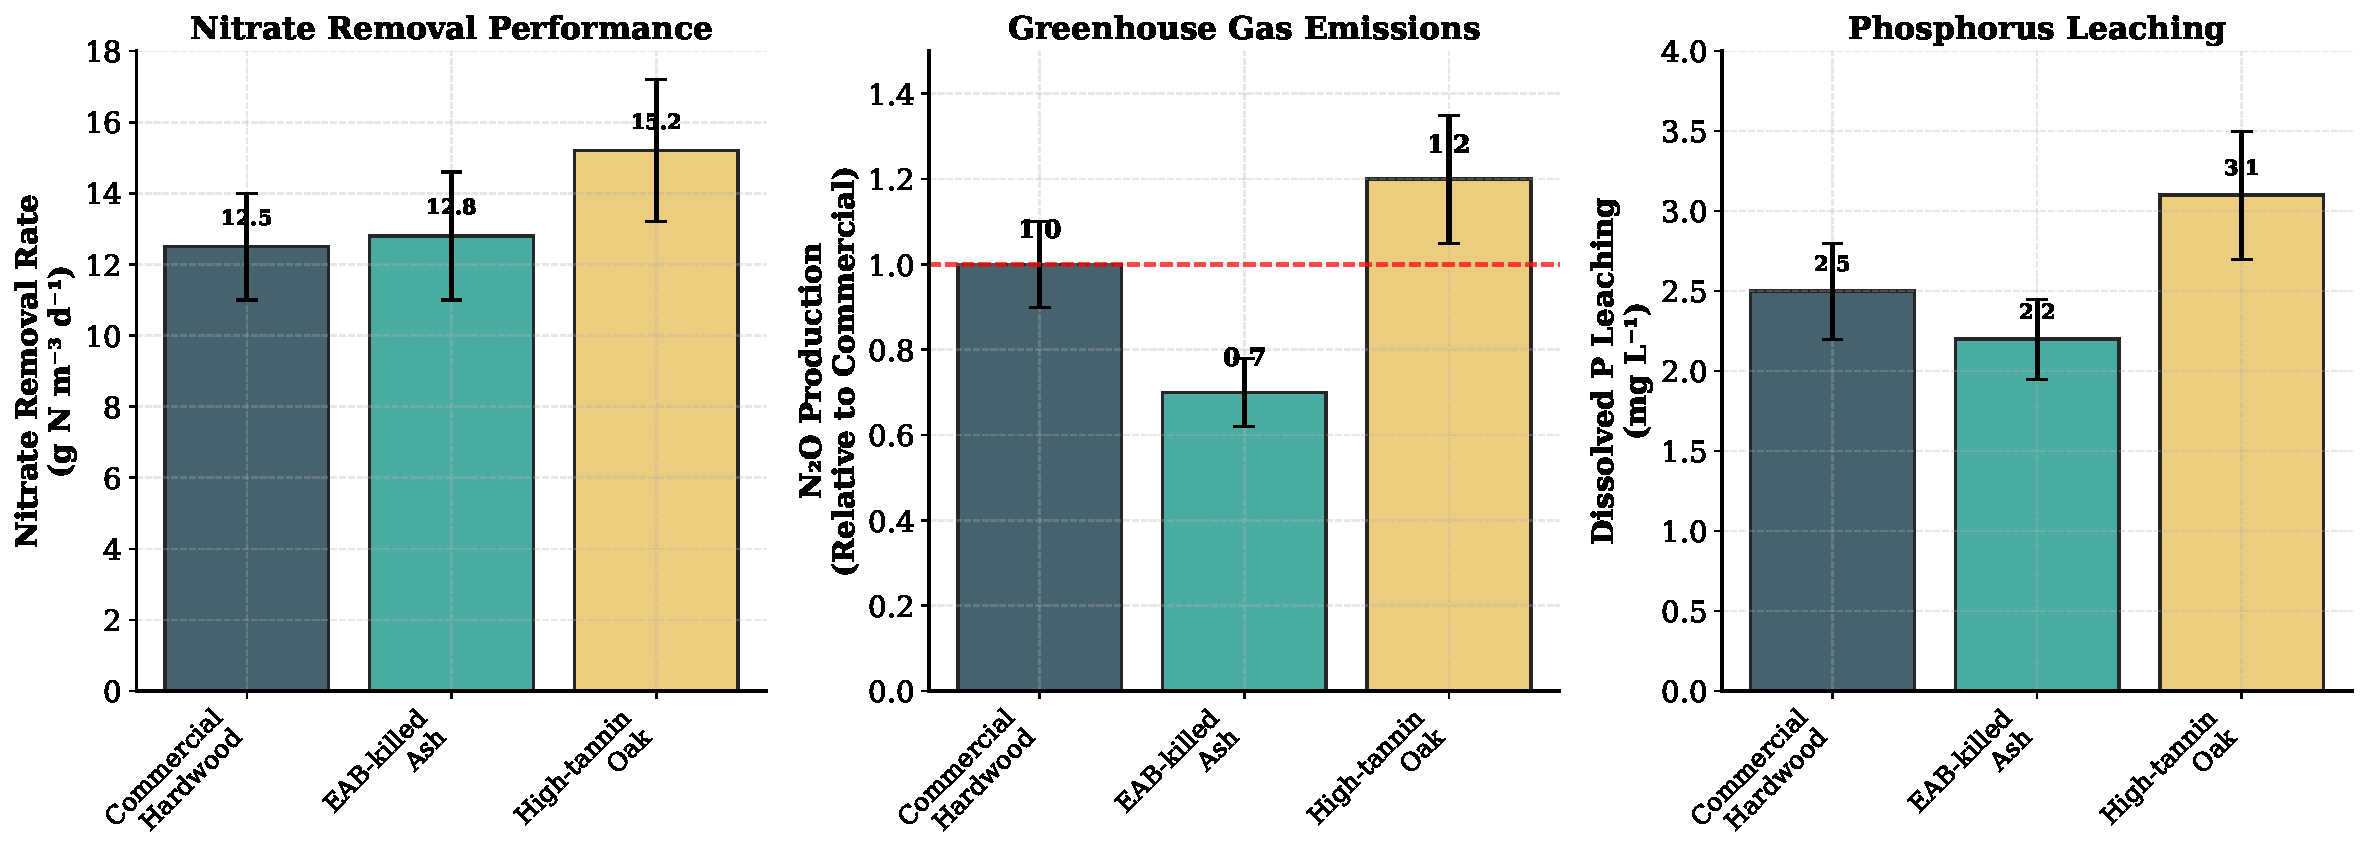
\includegraphics[width=0.8\textwidth]{fig9_wood_species_comparison_scientific}
\caption{Performance comparison of different wood species for bioreactor applications. EAB-killed ash shows comparable nitrate removal to commercial hardwood with lowest N$_2$O emissions. High-tannin oak demonstrates superior nitrate removal but higher greenhouse gas production. Data from Wickramarathne et al. 2021.}
\label{fig:wood_species_comparison}
\end{figure}

\subsection{Mixed Media and Amendments}

Mixed media approaches combining woodchips with other materials have demonstrated enhanced performance for multiple pollutants. Water treatment plant residuals (WTR) amended bioreactors achieved significantly greater removal efficiencies than woodchip-only systems for nitrate (33\% vs. 74\%), total phosphorus (28\% vs. 64\%), and dissolved reactive phosphorus (35\% vs. 89\%) during winter conditions \citep{RN625}. These systems also maintained high removal efficiencies (>80\%) for veterinary antibiotic compounds \citep{RN625}.

\subsection{Temperature Effects and Modeling}

Temperature significantly influences denitrification rates in woodchip bioreactors, with effects varying based on woodchip age and operating conditions \citep{RN228, RN242}. As shown in Figure \ref{fig:temperature_sensitivity}, temperature sensitivity varies considerably among different system configurations.

\begin{figure}[ht]
\centering
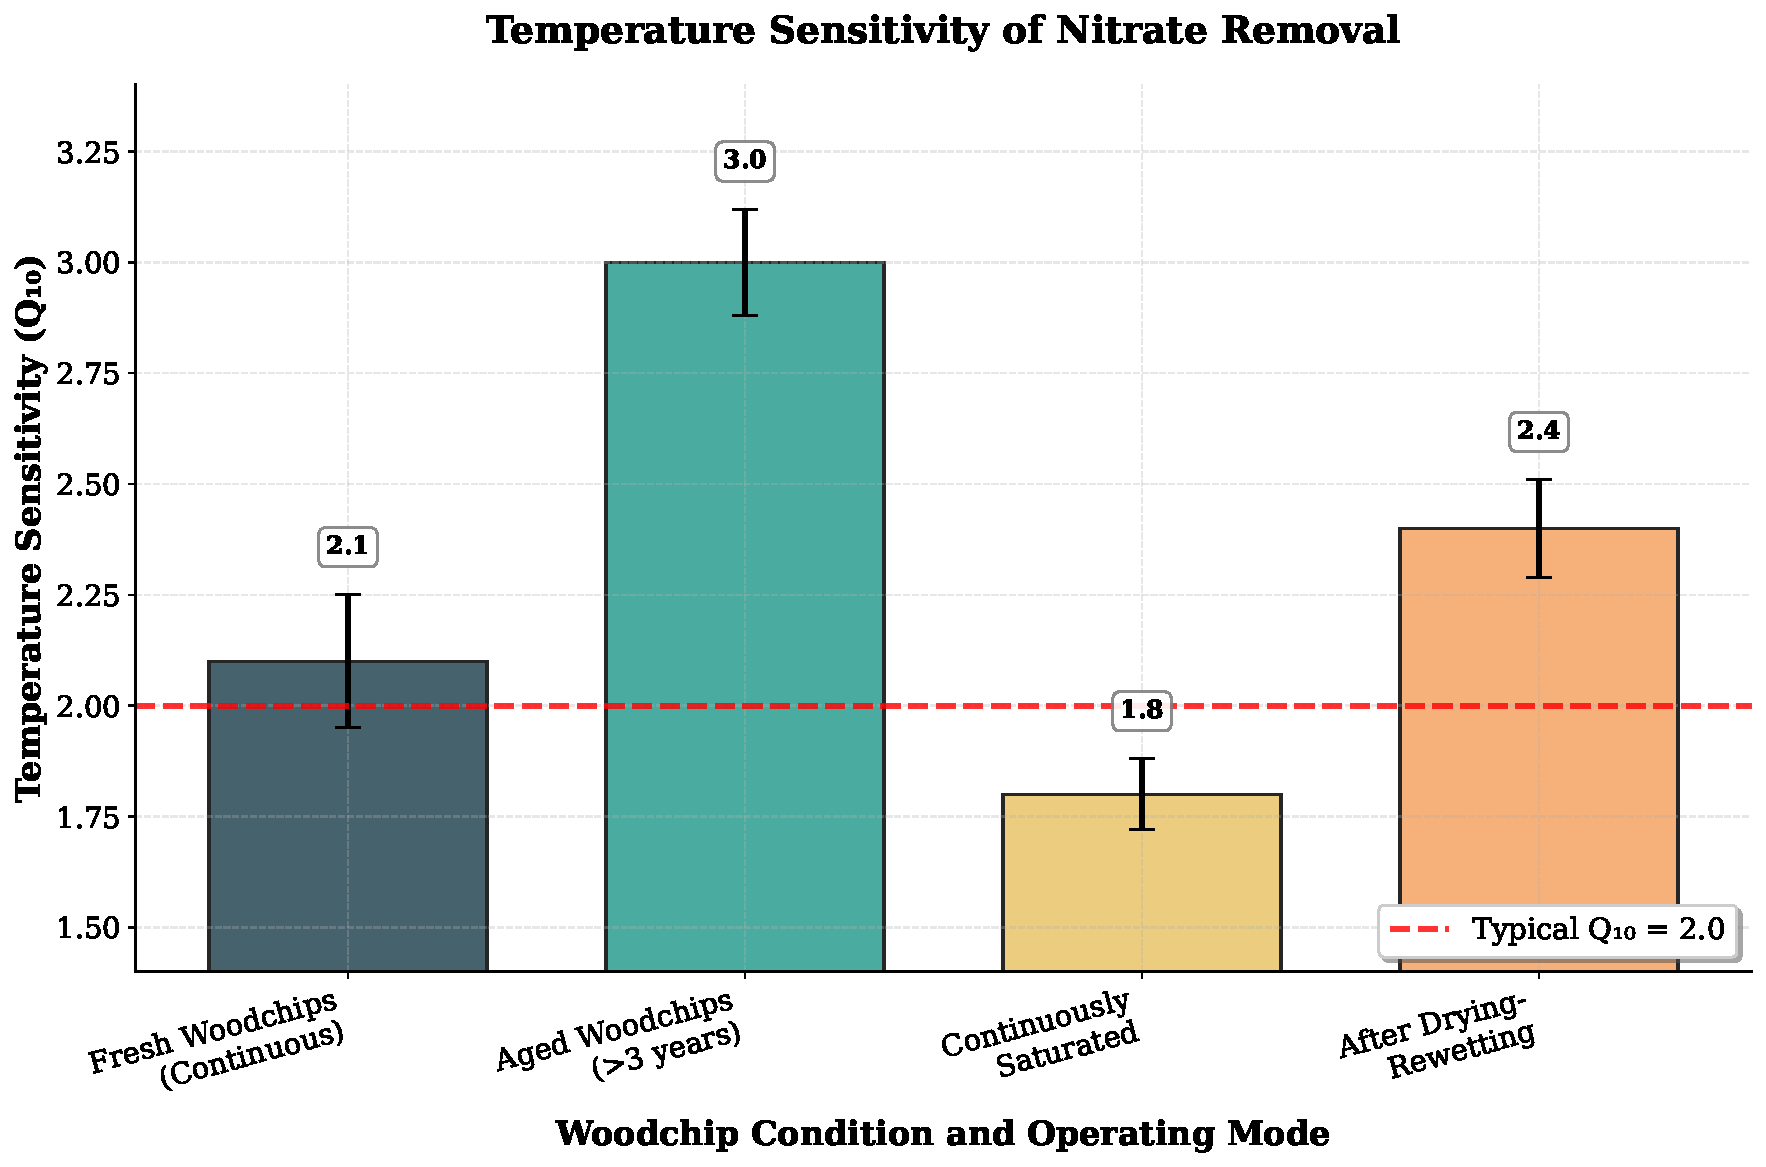
\includegraphics[width=0.8\textwidth]{fig4_temperature_scientific}
\caption{Temperature sensitivity (Q$_{10}$ values) of nitrate removal for different woodchip conditions and operating modes. Fresh woodchips show Q$_{10}$ = 2.1, aged woodchips >3 years show Q$_{10}$ = 3.0, continuously saturated operation shows Q$_{10}$ = 1.8, and after drying-rewetting cycles Q$_{10}$ = 2.4. Data from Maxwell et al. 2020.}
\label{fig:temperature_sensitivity}
\end{figure}

Advanced temperature modeling using simplified Arrhenius equations has provided quantitative frameworks for predicting bioreactor performance \citep{RN242}. Studies using column experiments at controlled temperatures (4-30°C) showed that temperature explained 45\% of the variance in measured nitrate removal rates and 40\% of the variance in dissolved organic carbon production rates. Above influent nitrate concentrations of 2 mg-N/L, nitrate removal could be effectively modeled as zero-order with temperature dependence using a temperature coefficient ($\theta$) of 1.16 ± 0.08 (95\% CI: 1.08-1.24) \citep{RN242}.

As illustrated in Figure \ref{fig:temperature_modeling}, mechanistic temperature models provide valuable tools for predicting bioreactor performance under varying thermal conditions.

\begin{figure}[ht]
\centering
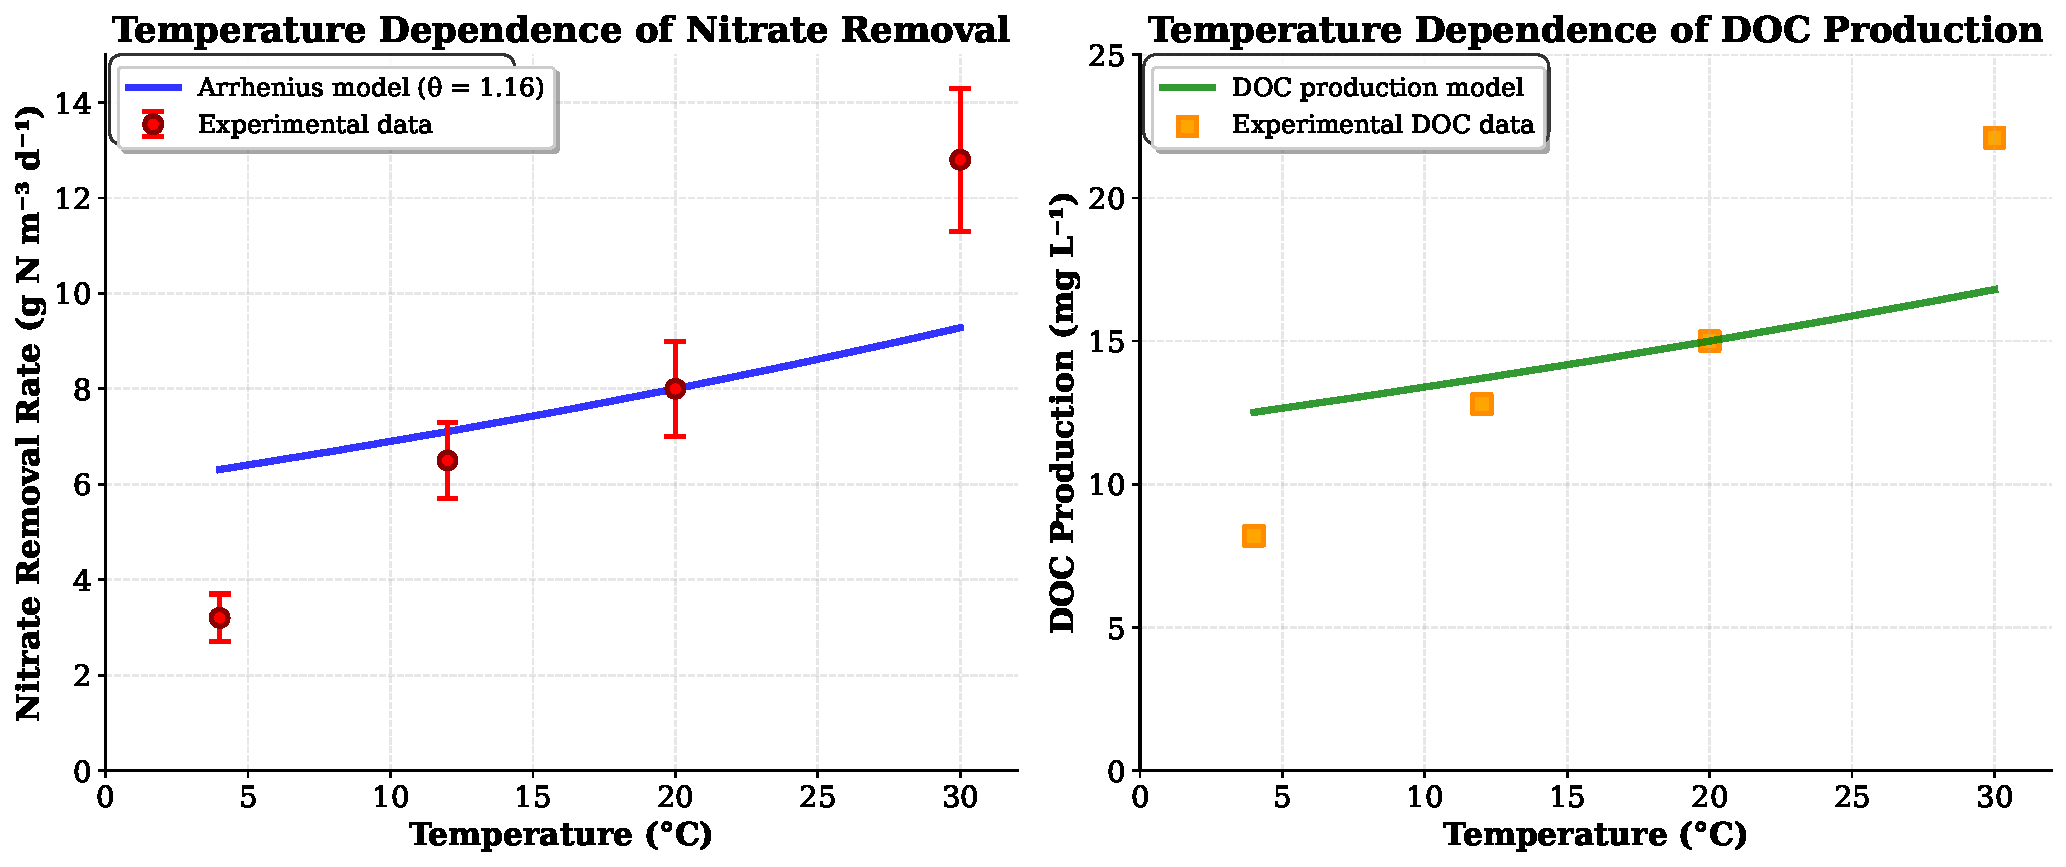
\includegraphics[width=0.8\textwidth]{fig10_temperature_modeling_scientific}
\caption{Temperature dependence modeling results showing Arrhenius model ($\theta$ = 1.16) validation against experimental data. Temperature explains 45\% of variance in nitrate removal rates and 40\% of variance in DOC production. Models enable performance prediction under varying thermal conditions. Data from Halaburka et al. 2017.}
\label{fig:temperature_modeling}
\end{figure}

\section{Performance Factors and Trade-offs}

\subsection{Scale Effects on Performance Relationships}

The relationship between nitrate removal rate and efficiency varies significantly across experimental scales \citep{RN312, RN310}. As shown in Figure \ref{fig:rate_vs_efficiency}, laboratory, pilot, and field-scale systems exhibit distinct patterns.

\begin{figure}[ht]
\centering
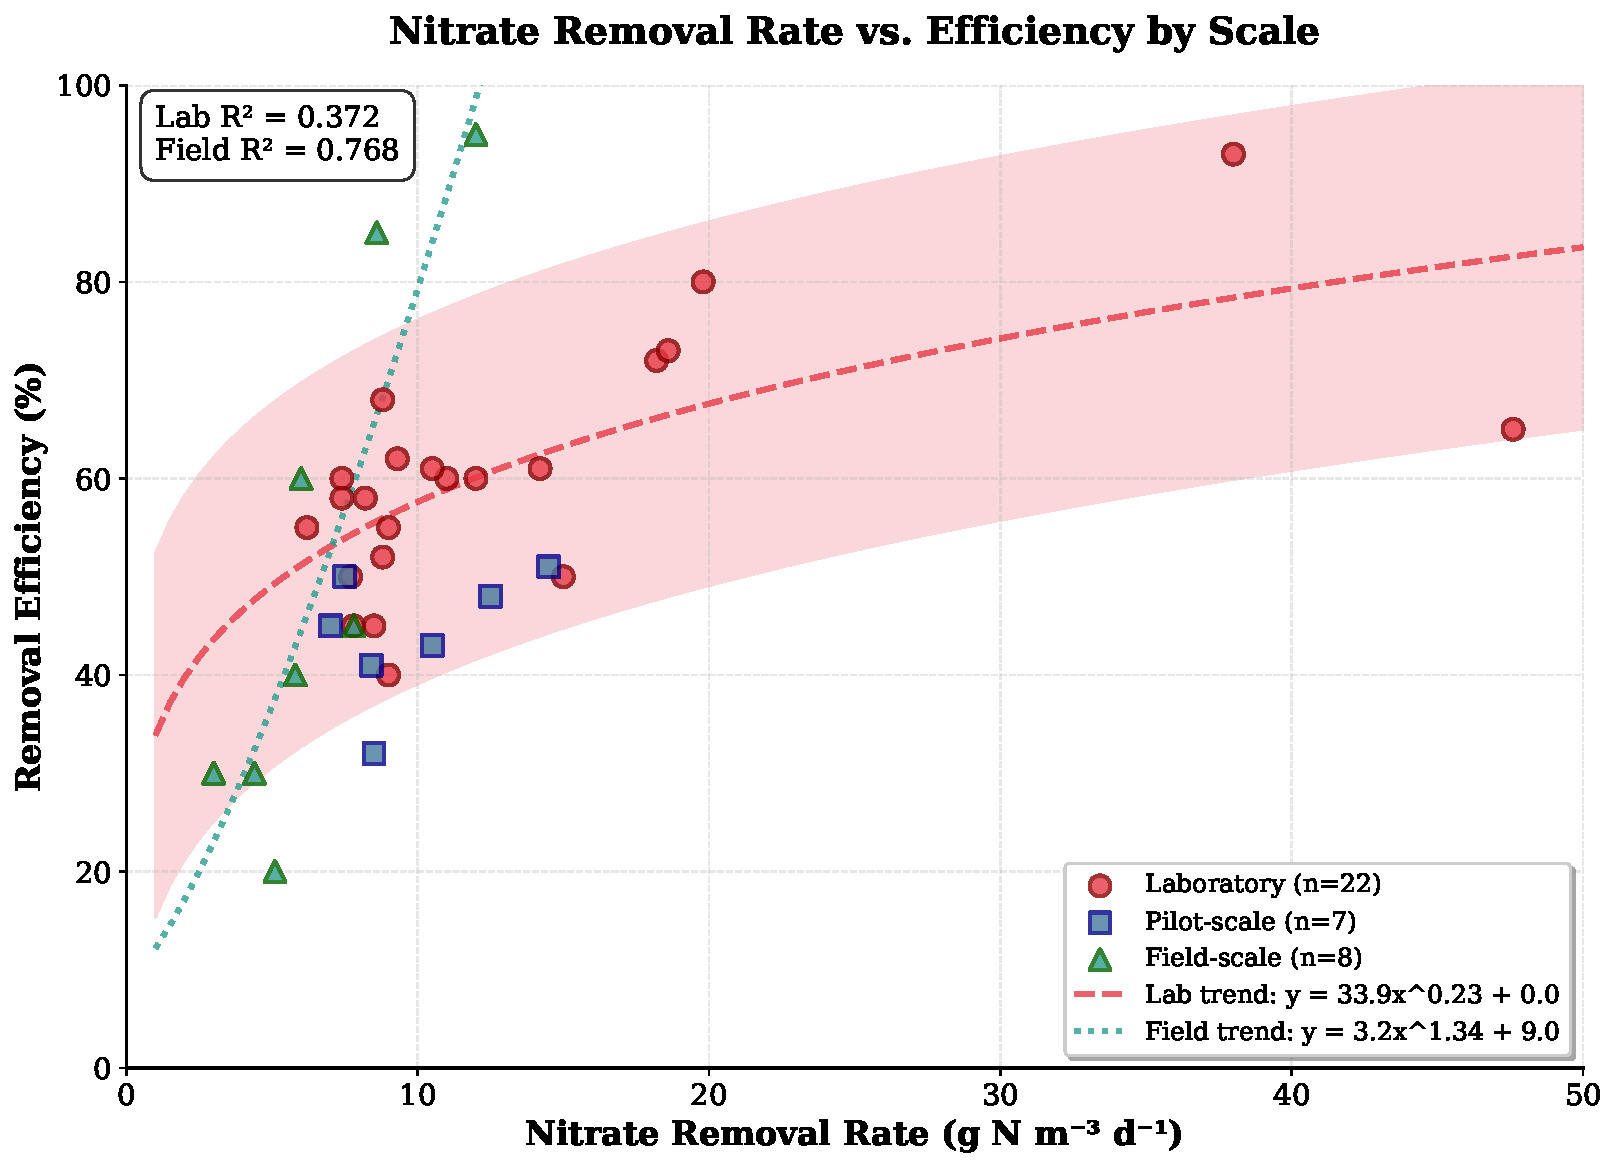
\includegraphics[width=0.8\textwidth]{fig2_rate_efficiency_scientific}
\caption{Relationship between nitrate removal rate and removal efficiency for different experimental scales. Laboratory data follows a logarithmic trend while field data shows a power relationship. The divergent relationships emphasize caution when applying laboratory-derived performance predictions to field applications.}
\label{fig:rate_vs_efficiency}
\end{figure}

Laboratory studies consistently achieve higher removal efficiencies at equivalent removal rates compared to field systems, likely due to controlled conditions \citep{new_ref_4}. Field systems face challenges including variable flow conditions, temperature fluctuations, seasonal changes in influent chemistry, and potential hydraulic short-circuiting that reduce overall treatment efficiency \citep{RN312, RN309}.

\subsection{Greenhouse Gas Emissions}

Denitrifying woodchip bioreactors can produce greenhouse gases, particularly nitrous oxide (N$_{2}$O) and methane (CH$_{4}$), as byproducts of microbial processes \citep{RN1181, new_ref_4}. N$_{2}$O is an obligate intermediate in the denitrification pathway; its emission occurs when the final reduction step to N$_{2}$ gas is incomplete. This can be caused by factors such as low pH, high nitrate concentrations, or fluctuating anoxic conditions. CH$_{4}$ is produced by methanogenic archaea, which thrive in highly reducing environments where more favorable electron acceptors like nitrate have been depleted. As shown in Figure \ref{fig:greenhouse_gas}, hydraulic retention time (HRT) strongly influences the production of both gases. Short HRTs can lead to incomplete denitrification and higher N$_{2}$O emissions, while very long HRTs can lead to nitrate depletion and subsequent methane production.

\begin{figure}[ht]
\centering
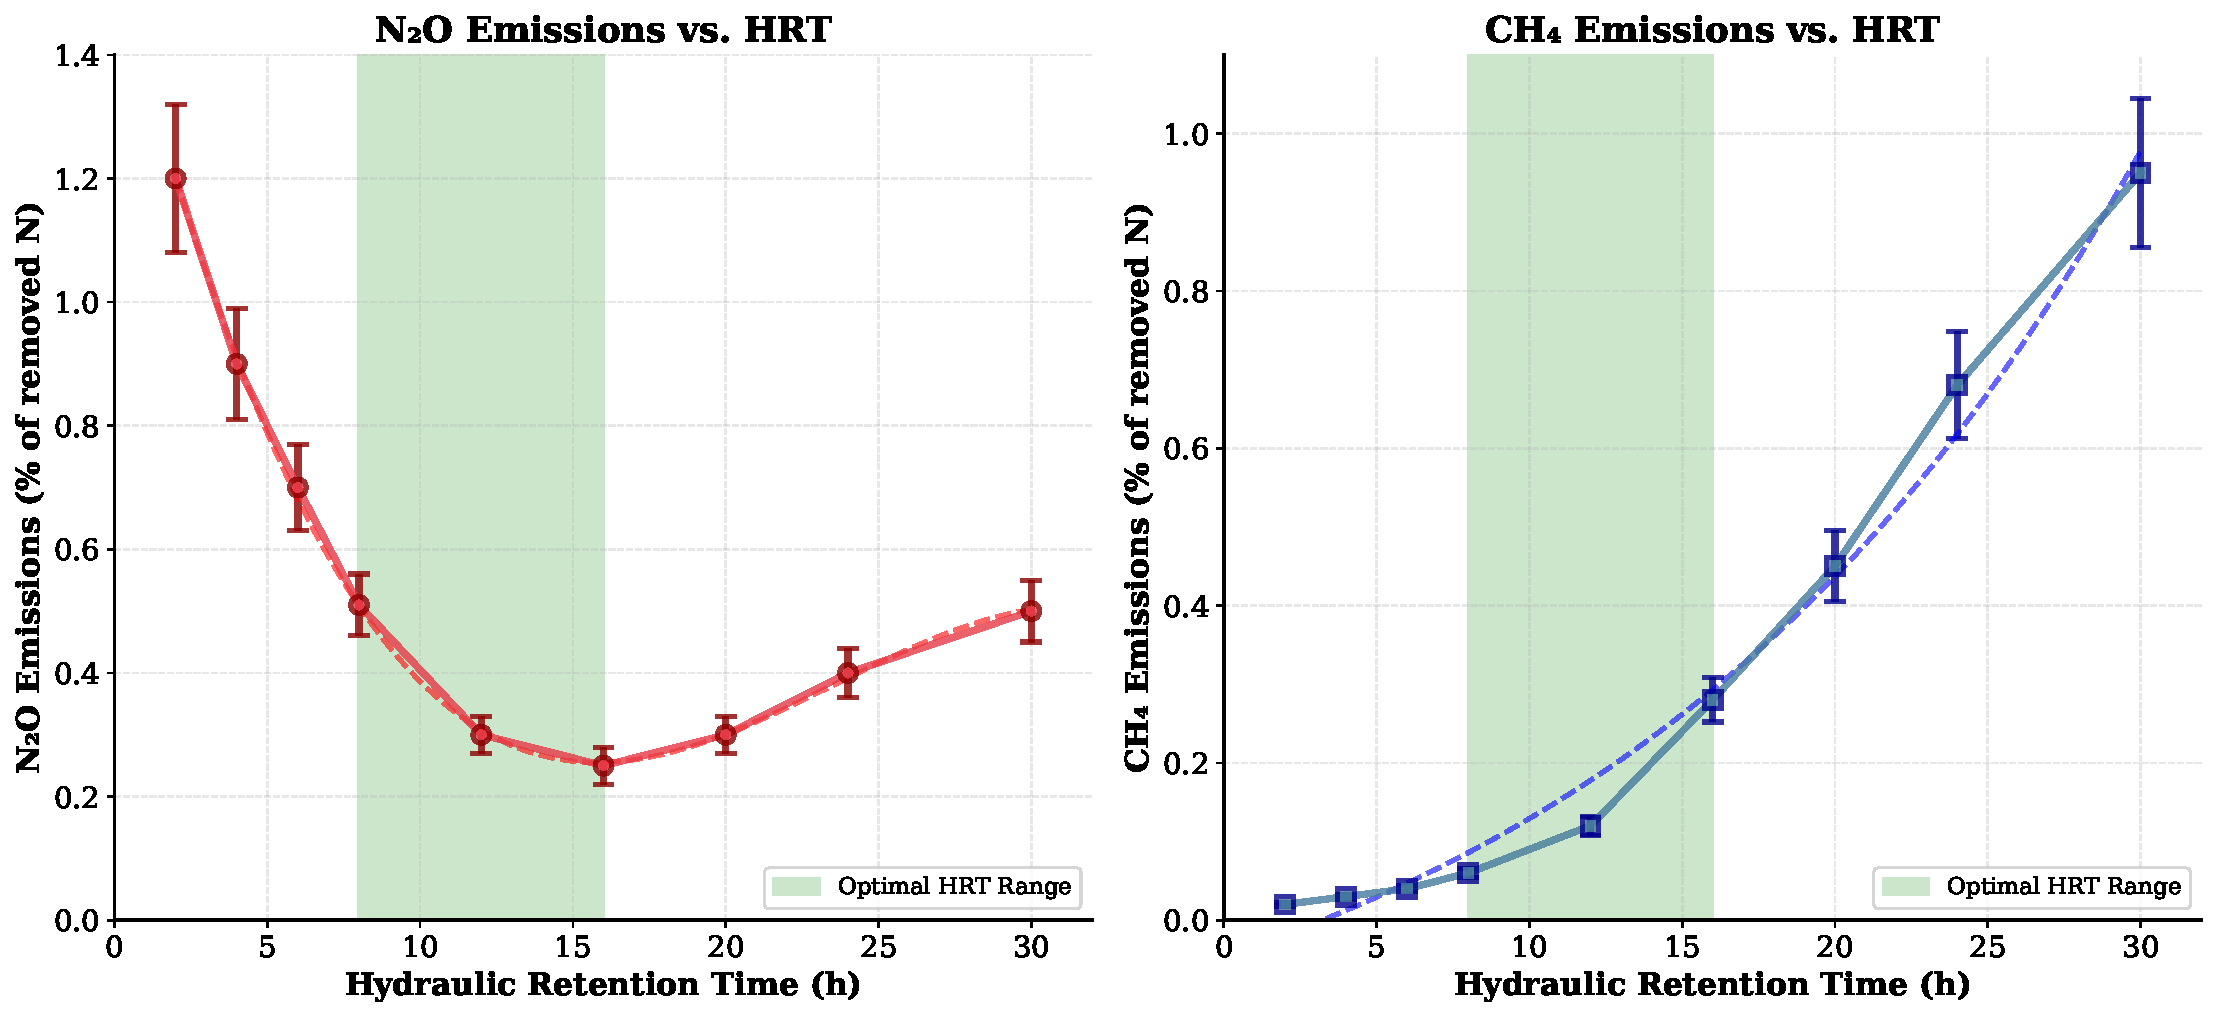
\includegraphics[width=0.8\textwidth]{fig6_greenhouse_gas_scientific}
\caption{Effect of hydraulic retention time on nitrous oxide and methane emissions from woodchip bioreactors. N$_2$O emissions decrease with longer HRT while CH$_4$ emissions increase substantially at longer HRTs due to developing methanogenic conditions. The optimal HRT range (8-16 hours) minimizes both emissions.}
\label{fig:greenhouse_gas}
\end{figure}

Recent field studies have provided important insights into greenhouse gas emissions from enhanced bioreactors. A comprehensive field study of an edge-of-field surface-flow bioreactor reported that N$_{2}$O emissions represented approximately 3.3-fold lower than the expected 0.75\% IPCC emission factor, indicating that well-designed bioreactors may not significantly swap aquatic nitrate pollution for atmospheric N$_{2}$O pollution \citep{RN1181}.

\subsection{Phosphorus Dynamics}

While primarily designed for nitrate removal, woodchip bioreactors significantly impact phosphorus dynamics \citep{RN625}. The woodchips themselves contain phosphorus, which can be leached during initial decomposition, often resulting in a net release of phosphorus during the start-up phase. As illustrated in Figure \ref{fig:phosphorus_removal}, phosphorus behavior varies considerably depending on media composition and operational phase.

\begin{figure}[ht]
\centering
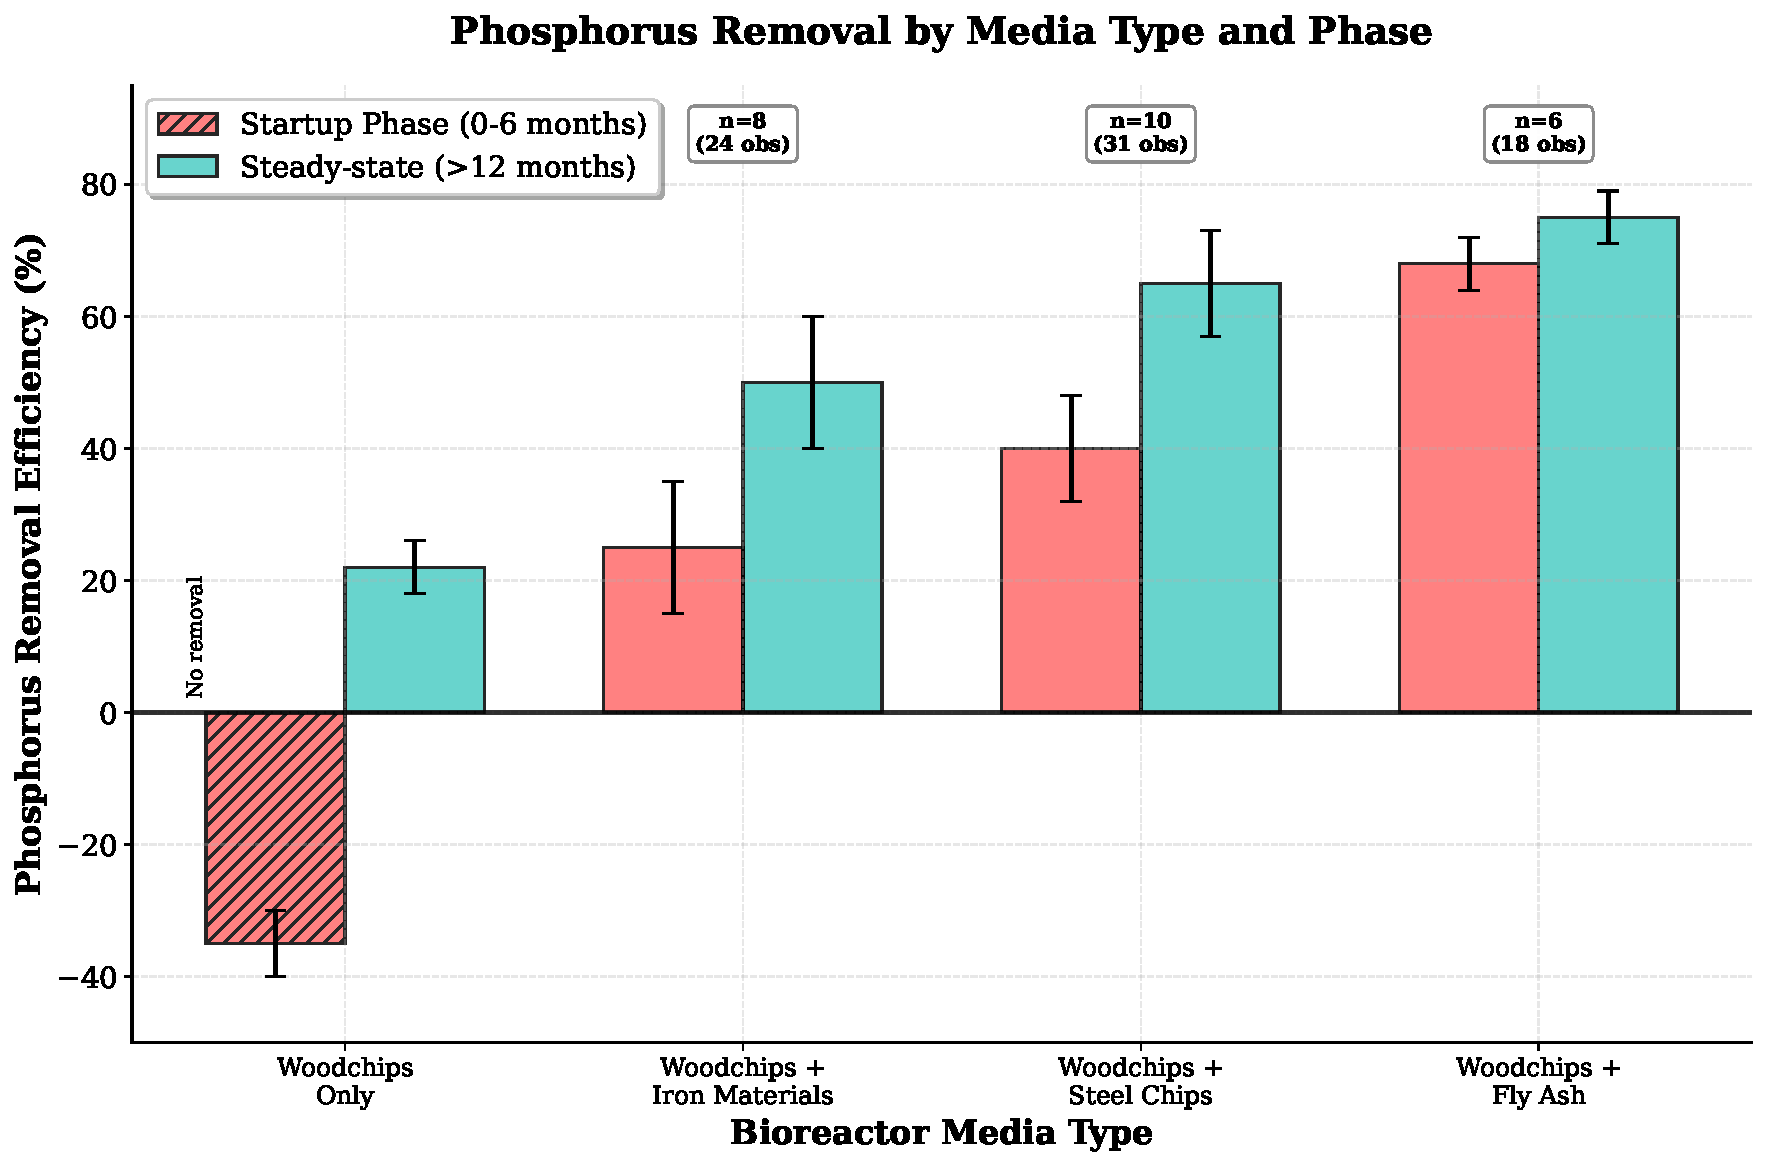
\includegraphics[width=0.8\textwidth]{fig7_phosphorus_scientific}
\caption{Phosphorus removal efficiency for different bioreactor media compositions during startup and steady-state operation phases. Woodchips-only systems initially release phosphorus but achieve modest removal in steady-state. Mixed media with metal-based additives show superior P removal. It should be noted that nitrate concentrations, which can affect overall microbial activity, were not consistently reported across these studies.}
\label{fig:phosphorus_removal}
\end{figure}

Standard woodchip bioreactors typically release phosphorus during the start-up phase, with leaching rates of 0.08-0.12 g P/m$^3$/day and negative removal efficiencies (approximately -35\%) \citep{RN625}. In contrast, media amended with materials containing iron, aluminum, or calcium can achieve significant phosphorus removal, primarily through adsorption and precipitation reactions. Metal-enhanced media significantly improve phosphorus removal, with woodchips combined with iron-based materials achieving 25-65\% P removal efficiency \citep{RN625}. In addition to these abiotic mechanisms, some studies suggest that biological phosphorus removal can occur through the activity of polyphosphate-accumulating organisms (PAOs), although this process is generally considered less significant in passive woodchip systems compared to engineered wastewater treatment plants.

\subsection{Dissolved Organic Carbon Leaching}

Dissolved organic carbon (DOC) leaching from woodchip bioreactors represents a potential water quality concern, particularly during start-up and following maintenance activities \citep{RN625, RN242}. As shown in Figure \ref{fig:doc_leaching}, DOC leaching varies considerably among media types and over time.

\begin{figure}[ht]
\centering
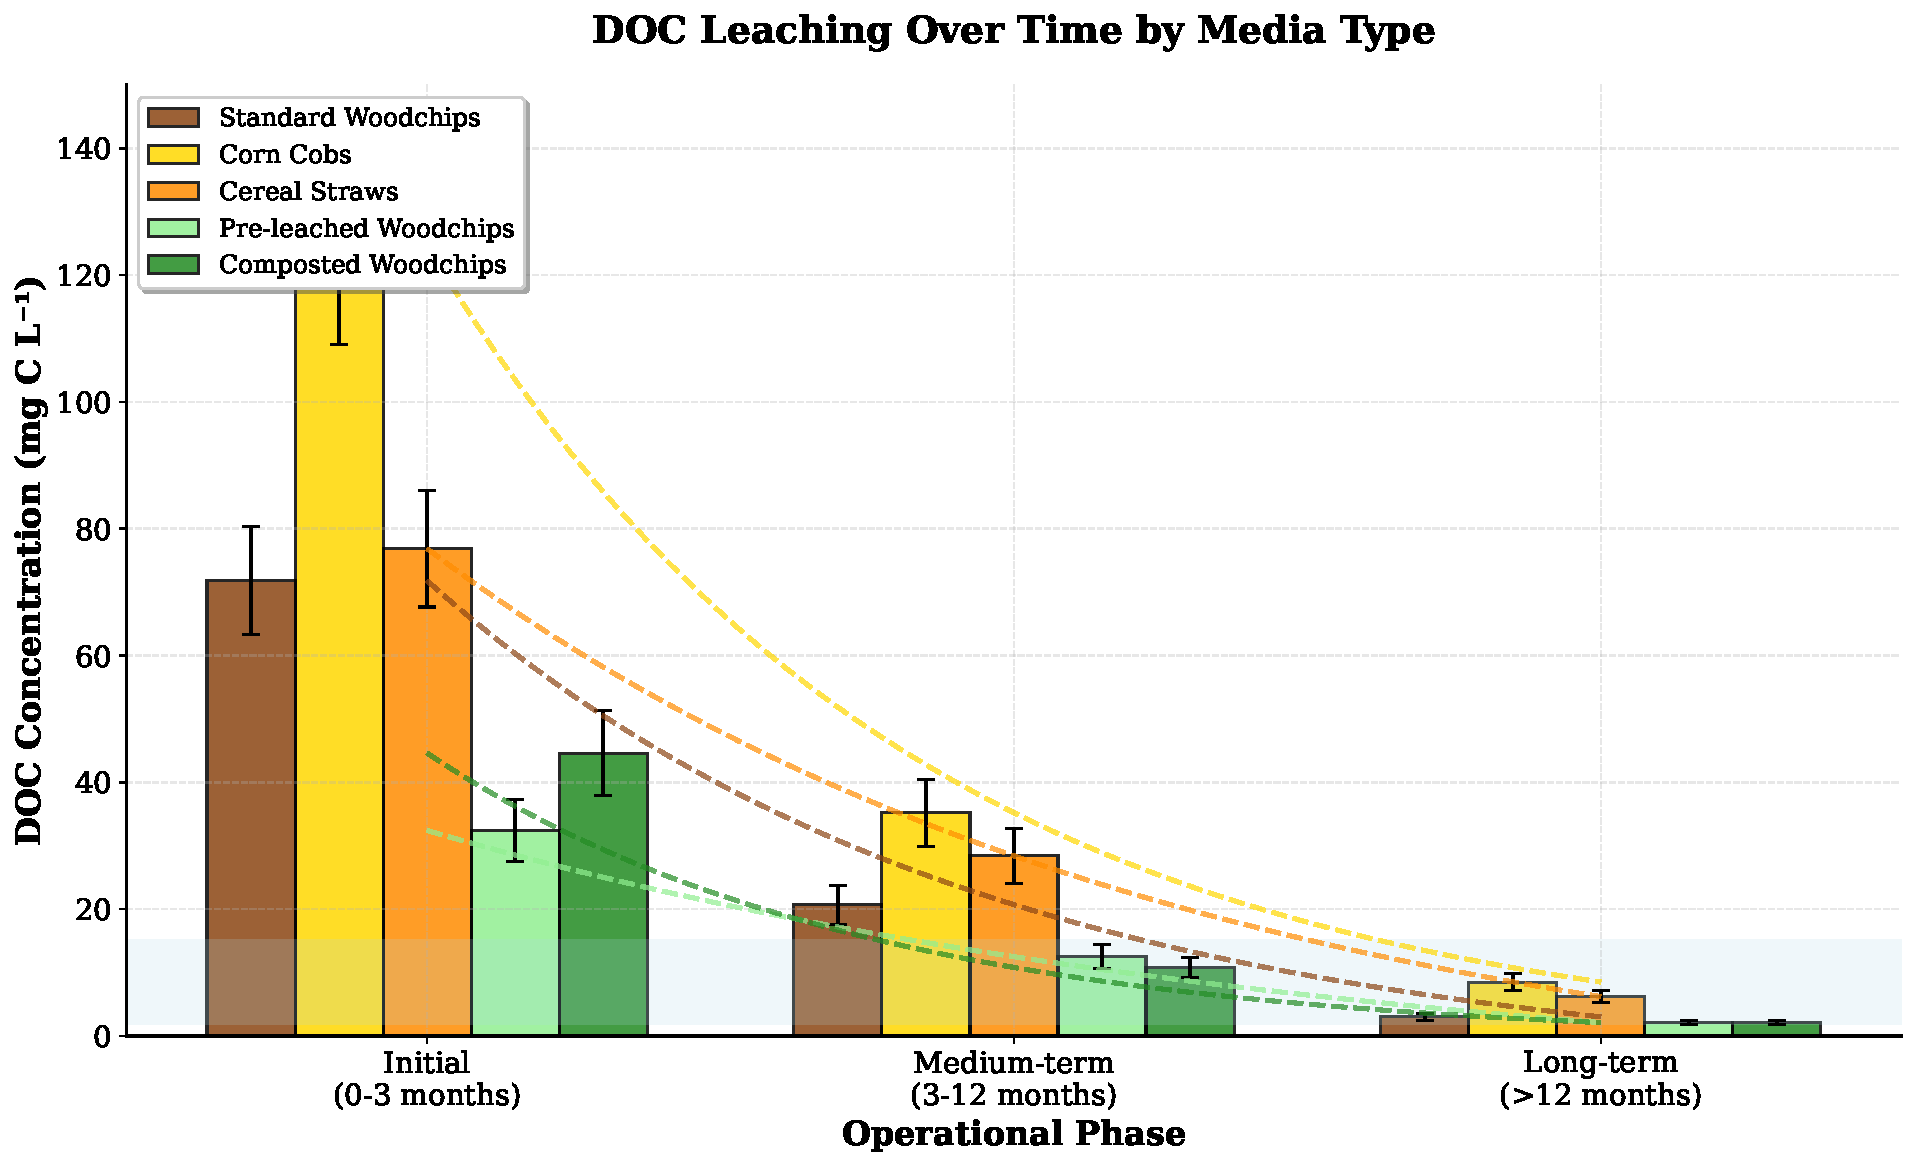
\includegraphics[width=0.8\textwidth]{fig8_doc_leaching_scientific}
\caption{Dissolved organic carbon leaching patterns for different media types and operational phases. Standard woodchips show decreasing DOC leaching over time. Alternative media show higher initial leaching but all decrease substantially over time.}
\label{fig:doc_leaching}
\end{figure}

Initial DOC leaching is substantial for all carbon-rich media, with standard woodchips releasing 71.8 mg DOC/L during the first 3 months of operation \citep{RN625}. However, DOC leaching decreases substantially over time for all media types, with standard woodchips declining to 20.7 mg/L after 3-12 months and further reducing to 3.0 mg/L in long-term operation \citep{RN625}.

\section{Economic Considerations and Cost-Effectiveness}

Enhanced woodchip bioreactors demonstrate varying cost-effectiveness depending on the enhancement strategy employed. Several comprehensive techno-economic analyses have provided quantitative assessments of different approaches, though costs vary significantly with geographic location, construction scale, and local economic conditions \citep{RN312, RN312}.

\subsection{Carbon Supplementation Costs}

Real-time acetate dosing systems achieved nitrate removal at a cost of \$86/kg N (2019 USD), with acetate cost being the main cost driver \citep{RN242}. This study evaluated biostimulation with 7.5 mg C/L acetate in a field-scale bioreactor in New York State, finding that the mass ratio of metabolized carbon to additional nitrogen removal was 2.5:1, though the total dosed C/N mass ratio was 5.1:1 due to incomplete acetate utilization. The high cost highlights opportunities for methods to improve acetate utilization efficiencies to enhance overall cost-effectiveness.

\subsection{Scale and Design Effects on Costs}

Techno-economic analyses of different bioreactor scales and configurations show that unit costs vary significantly with system design \citep{RN312}. Using a methodology that evaluated four scales of woodchip bioreactors operating at three hydraulic retention times (2, 8, and 16 hours), researchers found costs ranging from \$0.74 to \$60.13 per kg N removed (2020 USD). The lowest unit cost (\$0.74 kg$^{-1}$ NO$_3$-N removed) was achieved by large-scale bioreactors sized to minimize bypass flow at 16-hour HRT, while the highest unit cost (\$60.13 kg$^{-1}$ NO$_3$-N removed) occurred in pilot-scale bioreactors designed with bypass flow.

For pumped bioreactor systems, techno-economic analysis showed unit costs ranging from approximately \$5 to \$27 per kg NO$_3$-N removed for cistern and supplemental surface water bioreactors under most scenarios \citep{RN312}.

\subsection{Field-Demonstrated Costs}

Actual field construction costs have been documented for full-scale implementations. In Illinois, construction costs for eight full-scale bioreactors averaged \$12,250 ± \$7,520 across sites (2018 USD, equivalent to \$16,020 ± \$9,960 in 2023 price levels) \citep{RN312}. This study used actual construction costs obtained via invoices and personal communications, combined with monitored nitrate removal data from one to six years of monitoring per site. The cash-flow discounting procedure assumed two media recharges over a 24-year planning horizon. Monitored nitrate removal across 27 site-years resulted in a median cost of \$33/kg N removed annually. Drainage treatment area-based costs averaged \$132/ha-year, and treatment area was strongly correlated with capital costs (R$^2$ = 0.90; p = 0.001).

European costs appear higher, with Danish field-based bioreactors achieving nitrogen removal at approximately \$50 per kg N (2023 USD), which was 50\% higher than standard costs defined by Danish authorities \citep{RN312}. The cost efficiency analysis identified larger investments in the bioreactor itself combined with higher advisory costs as key cost drivers.

\subsection{Alternative Media Economics}

Alternative media approaches show promise for improved cost-effectiveness. A comprehensive 15-year cost assessment of mixed media systems found that 75\% corn cobs with 25\% woodchips (CC75) achieved costs of \$10.56 to \$13.89 per kg N removed, making it the most cost-efficient treatment \citep{new_ref_4}. This compared favorably to woodchips-only systems (\$13.30 to \$88.11 per kg N) and 25\% corn cobs with 75\% woodchips (\$22.41 to \$60.13 per kg N). The analysis used pilot-scale bioreactor data to estimate full-scale removal rates and costs, incorporating carbon treatments at hydraulic retention times of 2, 8, and 16 hours.

\subsection{Cost Analysis Limitations}

Cost estimates should be interpreted cautiously due to variations in methodology, included cost components (capital only vs. full lifecycle), temporal variations in pricing, and different economic assumptions across studies. Most cost assessments assume specific values for removal rates or operational parameters, and actual field performance may differ significantly from laboratory or modeled predictions. Additionally, many analyses do not include engineering design costs, which are becoming increasingly important for implementation \citep{RN312}.

\section{Design and Implementation Recommendations}

\subsection{Best Practices for Enhanced Systems}

Successful implementation of enhanced woodchip bioreactors requires careful attention to design details, construction practices, and operational management \citep{RN310, RN312}. For carbon supplementation approaches, automated dosing systems with real-time monitoring should be implemented when possible, carbon addition should be distributed across multiple injection points, and hydraulic performance monitoring is essential due to potential impacts on conductivity \citep{RN242}.

For alternative media approaches, consideration of material longevity is important. While corn cobs can maintain performance for several years, most alternative materials decompose more rapidly than woodchips, potentially requiring more frequent replacement \citep{new_ref_2}. Mixed media designs should maintain minimum 50\% woodchips by volume to ensure structural integrity and long-term performance \citep{new_ref_4}. The physical properties of the chosen media are also critical to hydraulic performance. Material particle size, shape, and tendency to compact will directly influence hydraulic conductivity, porosity, and the potential for preferential flow paths or short-circuiting.

Hydraulic optimization through proper aspect ratios and internal baffles can significantly improve treatment efficiency without additional operational costs \citep{RN309}. Studies have shown that aspect ratios between 3:1 and 5:1 (length to width) combined with strategically placed baffles can reduce short-circuiting and improve contact time \citep{RN309}.

\subsection{Monitoring and Performance Assessment}

Effective monitoring and performance assessment are essential for optimizing enhanced bioreactor function \citep{RN310, RN312}. Concentration-based metrics provide basic performance indicators, mass-based metrics offer comprehensive treatment assessment, and removal kinetics parameters provide process insight. Side effect assessment should include DOC, greenhouse gas, and phosphorus monitoring, particularly during start-up phases when leaching is highest \citep{RN625, RN1181}.

Enhanced bioreactor designs should not be implemented without proper monitoring systems at this stage of development. Adaptive management approaches that adjust operational parameters based on monitoring results can significantly improve long-term performance and environmental outcomes \citep{RN310}.

\section{Study Limitations and Future Research Directions}

\subsection{Limitations of Current Analysis}

This review has several important methodological limitations that should be considered when interpreting results. **Statistical Analysis Limitations**: Rather than conducting formal meta-analysis with standardized effect sizes and statistical testing, this review employs narrative synthesis due to substantial heterogeneity in study designs, operational conditions, and reporting metrics across the bioreactor literature. The comparative data presented (e.g., Figure \ref{fig:removal_rates_by_strategy}) should be interpreted as descriptive summaries rather than statistically validated comparisons. Future work should develop standardized protocols for bioreactor performance assessment to enable more rigorous quantitative synthesis.

**Study Selection and Heterogeneity**: While this review encompasses a broad range of enhancement strategies, the included studies vary substantially in experimental scale (laboratory vs. field), duration, influent characteristics, and measurement protocols. This heterogeneity limits the ability to draw definitive conclusions about relative effectiveness of different approaches. The majority of observations come from laboratory studies, which may not accurately reflect field performance due to controlled conditions and shorter operational periods \citep{RN312}.

**Geographic and Climatic Bias**: Studies are predominantly from North America and Europe, potentially limiting applicability to other regions with different climatic conditions or regulatory frameworks \citep{RN1023, RN258}. Temperature and seasonal effects may vary significantly in tropical or arid climates not well-represented in the current literature.

**Economic Analysis Limitations**: Cost analyses are particularly challenging to compare due to different economic conditions, included cost components (construction only vs. full lifecycle), temporal variations in pricing (studies span 2018-2023 without consistent inflation adjustment), and varying methodological assumptions. Many cost estimates are based on laboratory-scale performance extrapolations rather than actual field demonstrations \citep{RN312}.

**Publication and Selection Bias**: The review may favor studies reporting positive enhancement effects, as negative or inconclusive results are less likely to be published. Additionally, the emphasis on enhancement strategies inherently excludes studies focused solely on conventional bioreactor optimization.

**Temperature Modeling Limitations**: The reported temperature coefficient θ = 1.16 ± 0.08 and Q$_{10}$ values ranging from 1.8-3.0 require reconciliation \citep{RN242, RN228}. The relationship Q$_{10}$ = θ$^{10}$ means θ = 1.16 should correspond to Q$_{10}$ = 2.0, but observed Q$_{10}$ values suggest temperature sensitivity varies considerably with system conditions (woodchip age, saturation status, loading conditions). This highlights the need for more mechanistic understanding of temperature effects in enhanced systems.

**Scale-Up Validation Gap**: Laboratory studies consistently achieve higher removal efficiencies at equivalent removal rates compared to field systems (Figure \ref{fig:rate_vs_efficiency}). The mathematical relationships between laboratory and field performance remain poorly characterized, creating significant uncertainty when scaling enhancement strategies from laboratory to field applications \citep{RN312}.

\subsection{Future Research Priorities}

To advance the science and application of enhanced woodchip bioreactors, future research should be prioritized to address critical knowledge gaps. The following presents a structured outlook on key research areas:

\subsubsection{Field Validation and Standardization}
\begin{itemize}[leftmargin=*]
    \item \textbf{Long-Term Field Validation:} There is a pressing need for multi-year field trials of promising lab-scale enhancement strategies, especially for alternative media and bioaugmentation, to assess real-world performance, longevity, and operational challenges \citep{RN629}.
    \item \textbf{Standardized Protocols:} The development and adoption of standardized protocols for performance assessment are critical for cross-study comparisons. This includes consistent metrics for influent/effluent characterization, performance reporting, and uncertainty analysis \citep{RN310}.
    \item \textbf{Scale-Up Relationships:} Research is needed to quantify the relationships between lab, pilot, and field-scale performance to develop reliable models for scaling up enhancement strategies \citep{RN312}.
\end{itemize}

\subsubsection{Mechanistic Understanding and Optimization}
\begin{itemize}[leftmargin=*]
    \item \textbf{Temperature Modeling:} Refining temperature dependence models is crucial to reconcile the variability in reported Q$_{10}$ and $\theta$ values and to develop robust predictive tools for diverse operational conditions \citep{RN242, RN258}.
    \item \textbf{Carbon Utilization Efficiency:} Strategies to improve the efficiency of carbon supplementation are needed to reduce operational costs. For example, understanding the factors that led to only 49\% acetate utilization in one field trial could unlock significant cost savings \citep{RN242}.
    \item \textbf{Hybrid Systems:} Further investigation into hybrid systems that integrate bioreactors with other technologies (e.g., constructed wetlands, P-adsorbing filters) is warranted to develop comprehensive, multi-pollutant treatment trains \citep{RN625}.
\end{itemize}

\subsubsection{Broadening the Scope of Assessment}
\begin{itemize}[leftmargin=*]
    \item \textbf{Life-Cycle Assessment (LCA):} Comprehensive LCAs are needed to evaluate the full environmental footprint of enhancement strategies, including the impacts of producing and transporting carbon sources or other media amendments.
    \item \textbf{Climate Change Resilience:} The performance of enhanced systems should be evaluated under future climate scenarios, including projected changes in temperature and hydrology, to ensure their long-term viability \citep{RN1181}.
    \item \textbf{Maintenance and Decommissioning:} Research into the long-term maintenance needs, media replacement schedules, and end-of-life management of enhanced bioreactors is a critical but often overlooked area \citep{RN629}.
\end{itemize}

\section{Conclusions}

This systematic review confirms that enhancement strategies can substantially elevate the nitrate removal performance of woodchip bioreactors, transforming them into more potent and reliable treatment systems. The choice of enhancement is not a one-size-fits-all solution but rather a complex decision involving trade-offs between performance gains, operational complexity, economic costs, and environmental side effects.

The most significant performance boosts are achieved through carbon supplementation and the use of alternative media. These methods can increase nitrate removal rates by up to four-fold compared to conventional systems, with rates reaching as high as 38 g N/m$^3$/day. However, this comes at a cost, both economically (e.g., \$10-86 per kg N removed) and operationally, with potential impacts on hydraulic performance and the need for more frequent media replacement.

Environmental trade-offs, such as the emission of greenhouse gases and the leaching of phosphorus and dissolved carbon, are manageable. The evidence suggests that with proper design and operational control, such as optimizing hydraulic retention time, these "pollution swapping" risks can be mitigated, and in some cases, co-benefits like phosphorus removal can be achieved.

The path forward for enhanced bioreactors requires a concerted research effort focused on bridging the gap between laboratory potential and field reality. As outlined in the future research priorities, there is a critical need for long-term, field-scale validation of these enhancement strategies. Developing standardized protocols for performance and cost analysis is paramount for enabling robust comparisons and guiding practitioners. Ultimately, the successful implementation of enhanced bioreactors will depend on a holistic, site-specific approach that balances the desired level of treatment with local constraints and environmental goals. By continuing to refine these technologies and the frameworks for their assessment, enhanced woodchip bioreactors can play an increasingly vital role in addressing the global challenge of nitrate pollution.

\section{Acknowledgments}

The authors acknowledge that no specific funding was allocated for this project. Both authors contributed to this work as part of their ongoing research activities at their respective institutions.

\bibliographystyle{plainnat}
\bibliography{lit}

\end{document}